\chapter{Durchführung}
\label{chap:Durchfuehrung}

In der bereits hergeleiteten Theorie wird der Lösungsweg für das beschrieben Problem vorgestellt. Mit dem zur Verfügung gestelltem Skript, das auf dieser Theorie basiert wird nun die Parameterstudie durchgeführt. Um relevante Ergebnisse zu erlangen, müssen zuerst weitere Gleichungen in das Skript eingearbeitet werden.\\
In dem Skript wird eine Konstante $c$ als Vorfaktor für die Kraftberechnung aus dem Punktkontakt verwendet. Um die Berechnungsmöglichkeiten zu erweitern, wird $c$ nun durch eine Gleichung der Hertz'schen Pressung ersetzt, die wie folgt Hergeleitet wird:\\
Die Gleichung für die Hertz'sche Pressung eines Kugel-Kugel-Punktkontaktes lautet wie in Gleichung~\ref{form:ZvonP}

\begin{equation}
	\label{form:ZvonP}
	z(P) = \left[ \frac{9 P^{2} (1 - \nu^{2})^{2}}{2 E^{2}} \cdot \left( \frac{1}{2 r_{1}} + \frac{1}{2 r_{2}} \right) \right]^{\frac{1}{3}}
\end{equation}

Da einer der beiden Körper eine Platte mit dem Radius $r_{p} = \infty$ ist, folgt durch einsetzen von $r_{p}$ und umstellen nach P:

\begin{equation}
	\label{form:PvonZ}
	P(z) = \sqrt{\frac{4 r_{g}}{9}} \cdot \frac{E}{(1 - \nu^{2})} \cdot z^{\frac{3}{2}}
\end{equation}
	
Hier ist $\frac{E}{(1 - \nu^{2})}$ der reduzierte E-Modul, welcher durch Gleichung~\ref{form:redE} beschrieben wird.

\begin{equation}
	\label{form:redE}
	\frac{E}{(1 - \nu^{2})} = \left( \frac{(1 - \nu_{p}^{2})}{E_{p}} + \frac{(1 - \nu_{g}^{2})}{E_{g}} \right)^{-1}
\end{equation} 

Nun wird $c$ als Vorfaktor von $z^{\frac{3}{2}}$ in Gleichung~\ref{form:PvonZ} definiert, sodass folgt:

\begin{equation}
	\label{form:c}
	c = \sqrt{\frac{4 r_{g}}{9}} \cdot \frac{E}{(1 - \nu^{2})}
\end{equation}

Im Skript wurden Gleichungen~\ref{form:redE} und~\ref{form:c} unter den Konstanten implementiert und die einstellbaren Parameter der Platte und der Impaktor respektive um $E_{p}$ und $\nu_{p}$, bzw. $E_{g}$ und $\nu_{g}$ erweitert.\\

\section{Vorgehen und Vorbereitung}

Insgesamt wird das Problem durch die einstellbaren Parameter in Tabelle~\ref{tab:VariablenderStudie} beschrieben. In Anlehnung an \cite{Olsson.2000} wird das Massenverhältnis $Mr$ als einer der signifikanten Parameter gewählt. Davon ausgehend werden dann die anderen Parameter einzeln variiert und die Ergebnisse grafisch ausgewertet. 

\begin{table}[H]
	\begin{center}
		\caption{Variablen der Parameterstudie}
		\label{tab:VariablenderStudie}
		\begin{tabular}{l|c}
			\textbf{Variable} & \textbf{Bedeutung}\\
			\hline
			$a,b,h$ & Plattenmaße in [cm]\\
			$r_{g}$ & Impaktorradius in [cm]\\
			$v_{0}$ & Auftreffgeschwindigkeit [cm/s]\\
			$Mr$ & Massenverhältnis $\hat{=}$ $\frac{Impaktormasse}{Plattenmasse}$\\
			$\xi,\eta$ & Auftreffstelle des Impaktors\\
			$x,y$ & Auswertungsstelle\\		
		\end{tabular}
	\end{center}
\end{table}

\subsection{Auswertungskriterien und Annahmen}

Als Auswertungskriterien werden die Anzahl der einzelnen Schläge und der maximal auftretenden Kraft zusammen mit der Auslenkung der Platte gewählt. \\
Für die Studie werden folgende übergreifende Annahmen getroffen: 

\begin{enumerate}
	\item{Die Platte und der Impaktor sind isotrop, mit konstanten Stoffwerten}
	\item{Die Platte und der Impaktor sind aus identischem Material, mit gleichem E-Modul und Poissonzahl $\nu$}
\end{enumerate}

\subsubsection{Anzahl der Schläge}

Als Schlag wird hier ein Kraftverlauf bezeichnet, bei dem die Kraft $P_{i}$ zwischen den Schlägen auf Null fällt, nach der Bedingung in Gleichung~\ref{form:Schlagauftreten}:

\begin{equation} 
	\label{form:Schlagauftreten}
	F_{i-1} > 0 \; \wedge \; F_{i} = 0.0 
\end{equation}

Da im zeitlichen Verlauf auch nach dem ersten Auftreffen noch Schläge auftreten können, wird die Schrittanzahl auf $i = 1000$ gesetzt um signifikante Ergebnisse zu erlangen. 

\subsubsection{Maximale Auslenkung der Platte}

Die maximale Auslenkung $w_{max}$ wird direkt aus der Versuchsreihe ausgelesen und in Abhängigkeit des Massenverhältnisses und des zu veränderten Parameters dargestellt.

\subsubsection{Maximale Kraft}

Analog zur maximalen Auslenkung, wird die maximale Kraft $P_{max}$ direkt ausgelesen und in Abhängigkeit von $Mr$ und dem Parameter dargestellt.



\section{Parameterstudie}

Für die Parameterstudie wurde folgender Fall aus Ausgangspunkt gewählt: 

\begin{table}[H]
	\begin{center}
		\caption{Ausgangsfall Parameterstudie}
		\label{tab:Ausgang}
		\begin{tabular}{l|c}
			\textbf{Variable} & \textbf{Wert}\\
			\hline
			$a$ & 50.0 [cm]\\
			$b$ & 50.0 [cm]\\
			$h$ & 1.0 [cm]\\
			$r_{g}$ & 1.0 [cm]\\
			$v_{0}$ & 500.0 [cm/s]\\
			$\xi,\eta$ & 25.0 [cm]\\
			$x,y$ & 25.0 [cm]\\ 		
		\end{tabular}
	\end{center}
\end{table}

$Mr$ wird hier bewusst ausgelassen, da bei jedem Parameter außer der Auftreffstelle über das Massenverhältnis iteriert wird und dadurch kein Anfangswert, sondern eine Menge benötigt wird. Die Menge der $Mr$ ist nach Gleichung~\ref{form:Mr}:

\begin{equation}
	\label{form:Mr}
	0.01 \leq Mr \leq 2.50 \; , \;\; \mbox{Schrittweite:} \; \Delta Mr = 0.01
\end{equation}

Die Stoffparameter sind im Rahmen der Studie konstant und in Tabelle~\ref{tab:Stoff} definiert.

\begin{table}[H]
	\begin{center}
		\caption{Stoffparameter: Kugel und Platte}
		\label{tab:Stoff}
		\begin{tabular}{l|c}
			\textbf{Variable} & \textbf{Wert}\\
			\hline
			$E_{p}$ & $2.2 \cdot 1e06$ [$kg/cm^2$]\\
			$\nu_{p}$ & 0.3 [-]\\
			$\rho_{p}$ & 0.00796 [$kg/cm^{3}$]\\
			\hline
			$E_{g}$ &  $2.2 \cdot 1e06$ [$kg/cm^2$]\\
			$\nu_{g}$ & 0.3 [-]\\		
		\end{tabular}
	\end{center}
\end{table}

\subsection{Höhe der Platte}

Als erster Parameter wird die Höhe nach Gleichung~\ref{form:DeltaH} variiert. Alle anderen Werte werden nach Tabelle~\ref{tab:Ausgang} konstant gehalten.

\begin{equation}
	\label{form:DeltaH}
	0.5 [cm] \leq h \leq 2.5 [cm], \; \; \mbox{Schrittweite:} \; \Delta h = 0.1 [cm]
\end{equation}

Wenn man die Höhe, das Massenverhältnis und die Anzahl der Schläge aufträgt, ergibt sich Abbildung~\ref{fig:Hoehe}.

\begin{figure}[H]
	\begin{center}
		\begin{overpic}[width=\linewidth]{pictures/gnuplot/3d/Hoehe/production/Hoehe.eps}
			\put(45,4){Höhe [cm]}
			\put(18,30){\rotatebox{90}{Mr [-]}}
			\put(83,60){Aufschläge [-]}
		\end{overpic}
	\caption{Höhe, Mr und Anzahl der Aufschläge}
	\label{fig:Hoehe}
	\end{center}
\end{figure}

Man kann direkt ablesen, dass mehrere Aufschläge vermehrt im unteren Höhenbereich auftreten. Dies ist direkt auf die Steifigkeit der Platte zurückzuführen. Bei größerer Plattendicke ist die Steifigkeit der Platte größer und die Kugel prallt ab, ohne vermehrt aufzutreffen. Bei $h = 0.6 [cm]$ treten bis zu 10 Schlägen auf. Interessant ist auch, dass sich drei Bereiche in Abhängigkeit des Massenverhältnisses ausbilden. \\
Es ist offensichtlich, dass bei einem Massenverhältnis $Mr \geq 1.7$ und einer Plattendicke von $h \geq 1.6 [cm]$ nur noch einzelne Stöße auftreten. Hier ist anzunehmen, dass der elastische Stoßvorgang der Kugel ausreichend kinetische Energie entgegen der Stoßrichtung überträgt, dass sie sich schneller entfernt, als die Platte auslenken kann. \\
Auch bei der Auslenkung stimmen die Ergebnisse mit den Erwartungen überein. In Abbildung~\ref{fig:HoeheAuslenkung} ist zu erkennen, dass mit zunehmender Höhe die Auslenkung abfällt, da die Steifigkeit der Platte zunimmt. Die Steigung der Auslenkungskurve flacht mit zunehmendem $Mr$ ab. Am signifikantestem ist die Steigung im Bereich $0.01 \leq Mr \leq 1$. Ergo ist der Einfluss des Massenverhältnisses am größten in diesem Bereich.\\
Bei Plattendicken von $h \geq 1.3 [cm]$ flacht die Steigung der maximalen Auslenkung in einen annähernd linearen Bereich ab. Daher liegt nahe, dass die Höhe im Bereich bis $h = 1.3 [cm]$ den stärksten Einfluss hat.\\

\begin{figure}[h!]
	\begin{center}
		\begin{overpic}[width=\linewidth]{pictures/gnuplot/3d/Hoehe/production/HoeheAuslenkung.eps}
			\put(45,4){Höhe [cm]}
			\put(18,30){\rotatebox{90}{Mr [-]}}
			\put(83,60){Auslenkung [cm]}
		\end{overpic}
	\caption{Höhe, Mr und Auslenkung}
	\label{fig:HoeheAuslenkung}
	\end{center}
\end{figure}

Die größte Auslenkung tritt bei einem Massenverhältnis von $Mr = 2.5$ und einer Höhe von $h = 0.5 [cm]$ auf und beträgt $w(0.5,2.5) = 2.265 [cm]$, während die geringste Auslenkung bei $Mr = 0.01$ und $h = 2.5 [cm]$ mit $w = 0.0165 [cm]$ auftritt.\\
\\
Wenn man die maximal auftretende Kraft betrachtet, ergibt sich Abbildung~\ref{fig:HoeheKraft}.\\
Aus der maximalen Auslenkung kann man schlussfolgern, dass die maximale Kraft dort auftritt, wo die Auslenkung am geringsten ist, da hier am wenigsten Energie in die Deformation der Platte übergeht.\\
Bei $Mr = 2.5$ und $h = 2.5 [cm]$ tritt daher eine Kraft von $P = 598.36 [kN]$ auf. Die hier auftretende Kraft ist etwa um den Faktor $50$ größer als die geringste Kraft, die wie zu erwarten bei $Mr = 0.01$ und $h = 0.5 [cm]$ auftritt und $P = 10.88 [kN]$ beträgt. \\
Interessant zu betrachten ist auch, wie die Kraft mit größer werdendem $Mr$ zunimmt. Bei $h_{min} = 0.5 [cm]$ ist die Kraft bei $Mr_{max} = 2.5$ nur um den Faktor 2 größer als bei $Mr_{min} = 0.01$. Betrachtet man allerdings $h_{max} = 2.5 [cm]$, ist die Kraft bei $Mr_{max} = 2.5$ um den Faktor $14.4$ größer als bei $Mr_{min} = 0.01$, bzw. betragen die Kräfte $P_{max}(h_{max}) = 598.36[kN]$ und $P_{min}(h_{max}) = 41.4[kN]$.

\begin{figure}[H]
	\begin{center}
		\begin{overpic}[width=\linewidth]{pictures/gnuplot/3d/Hoehe/production/HoeheKraft.eps}
			\put(45,4){Höhe [cm]}
			\put(18,30){\rotatebox{90}{Mr [-]}}
			\put(80,62){Kraft [N]}
		\end{overpic}
	\caption{Höhe, Mr und Kraft}
	\label{fig:HoeheKraft}
	\end{center}
\end{figure}



\subsection{Geschwindigkeit des Impaktors}

Als nächster Parameter wird die Geschwindigkeit betrachtet. Da hier nur der Low-Velocity Bereich betrachtet wird, wird die Geschwindigkeit nach Gleichung~\ref{form:DeltaV0} variiert. Da sich bei der Geschwindigkeit beim Erstellen der Abbildungen signifikante Interpolationsfehler ergeben, wird hier bewusst eine andere Darstellungsweise verwendet, welche die Daten genauer wiedergibt. 

\begin{equation}
	100 [cm/s] \leq v_{0} \leq 1000 [cm/s] \; , \;\; \mbox{Schrittweite:} \; \Delta v_{0} = 10 [cm/s]
	\label{form:DeltaV0}
\end{equation}

Analog zur Höhenvariation wird zuerst die Anzahl der Aufschläge aufgetragen. In Abbildung~\ref{fig:Speed} ist zu erkennen, dass die Geschwindigkeit bei gleichbleibendem $Mr$ keinen Einfluss auf die Anzahl der Aufschläge hat. 

\begin{figure}[h!]
	\begin{center}
		\begin{overpic}[width=\linewidth]{pictures/gnuplot/3d/Speed/production/Speed.eps}
			\put(35,-1){Geschwindigkeit [cm/s]}
			\put(1,33){\rotatebox{90}{Mr [-]}}
			\put(90,70){Aufschläge [-]}
		\end{overpic}
		\caption{Geschwindigkeit, Mr und Anzahl der Aufschläge}
		\label{fig:Speed}
	\end{center}
\end{figure}

Die aus den Stößen resultierende Auslenkung wird in Abbildung~\ref{fig:SpeedAuslenkung} dargestellt. Man kann erkennen, dass der Einfluss des Massenverhältnisses mit zunehmender Geschwindigkeit zunimmt. \\
Die geringste Auslenkung tritt bei $Mr = 0.01$ und $v_{0} = 100 [cm/s]$ auf und beträgt $w = 0.008899 [cm]$, während die größte Auslenkung wie zu erwarten bei $v_{0,max} = 1000 [cm/s]$ und $Mr_{max} = 2.5$ berechnet wird und $w_{max} = 2.57 [cm]$ beträgt. \\
Auch zu sehen ist, dass im höheren Geschwindigkeitsbereich die Auslenkung stärker mit größer werdendem $Mr$ ansteigt. \\
Betrachtet man den Faktor der zwischen der $w_{min}(v_{0,min})$ und $w_{max}(v_{0,max})$ bei gegebenem $Mr$ liegt ist zu erkennen, dass die Geschwindigkeit im Zusammenspiel mit $Mr$ einen großen Einfluss auf die Auslenkung hat. Bei $v_{0,min}$ ist der Faktor mit $28.72$ fast gleich wie bei $v_{0,max}$ mit $29.72$.

\begin{figure}[H]
	\begin{center}
		\begin{overpic}[width=\linewidth]{pictures/gnuplot/3d/Speed/production/SpeedAuslenkung.eps}
			\put(35,-1){Geschwindigkeit [cm/s]}
			\put(1,33){\rotatebox{90}{Mr [-]}}
			\put(90,70){Auslenkung [cm]}
		\end{overpic}
		\caption{Geschwindigkeit, Mr und Auslenkung}
		\label{fig:SpeedAuslenkung}
	\end{center}
\end{figure}

Als letztes wird nun die Kraft aufgetragen. In Abbildung~\ref{fig:SpeedKraft} sind ähnliche Trends wie in Abbildung~\ref{fig:SpeedAuslenkung} zu sehen. \\
Auch hier nimmt die auftretende Kraft mit $v_{0}$ zu. Je größer $Mr$ hierbei ist, desto steiler die Kraftzunahme. Besonders deutlich wird dies, wenn man wieder die Faktoren zwischen $P_{max}$ und $P_{min}$ bei gegebenem $Mr$ und $v_{0}$ untersucht. \\
Bei $v_{0,min} = 100 [cm/s]$ ist $P(Mr_{min}) = 2.883 [kN]$ und damit um den Faktor $9.375$ kleiner als $P(Mr_{max}) = 27.063 [kN]$.\\
Bei $v_{0,max} = 1000 [cm/s]$ ist $P(Mr_{min}) = 38.892 [kN]$ und $P(Mr_{max}) = 282.326 [kN]$. Damit ist der Faktor hier $7.259$, allerdings liegt eine Größenordnung zwischen der Kraft bei $v_{0,min}$ und der Kraft bei $v_{0,max}$.

\begin{figure}[H]
	\begin{center}
		\begin{overpic}[width=\linewidth]{pictures/gnuplot/3d/Speed/production/SpeedKraft.eps}
			\put(35,-1){Geschwindigkeit [cm/s]}
			\put(1,33){\rotatebox{90}{Mr [-]}}
			\put(90,70){Kraft [N]}
		\end{overpic}
		\caption{Geschwindigkeit, Mr und Kraft}
		\label{fig:SpeedKraft}
	\end{center}
\end{figure}

\subsection{Impaktorradius}

Im Folgenden wird der Radius des Impaktors betrachtet. Nach Gleichung~\ref{form:Radius} wird der Radius der Kugel erhöht.

\begin{equation}
	0.5 [cm]\leq r_{g} \leq 10 [cm], \; \; \mbox{Schrittweite:} \; \Delta r_{g} = 0.1 [cm]
	\label{form:Radius}
\end{equation}

In Abbildung~\ref{fig:Radius} ist zu erkennen, dass der Radius nur einen geringen Einfluss auf die Anzahl der Aufschläge hat.\\
Bildet man die Daten in 3D ab, erkennt man leicht, dass die Anzahl der Aufschläge sich nur mit $Mr$ verändert. \\

\begin{figure}[H]
	\begin{center}
		\begin{overpic}[width=\linewidth]{pictures/gnuplot/3d/Radius/production/Radius.eps}
			\put(44,4){Radius [cm]}
			\put(18,30){\rotatebox{90}{Mr [-]}}
			\put(83,60){Aufschläge [-]}
		\end{overpic}
		\caption{Radius, Mr und Anzahl der Aufschläge}
		\label{fig:Radius}
	\end{center}
\end{figure}

Ähnliche Ergebnisse werden auch bei der Auslenkung erreicht. Wie in Abbildung~\ref{fig:RadiusAuslenkung} zu sehen ist, nimmt die Auslenkung nur bei hohen $Mr$ auch mit durch Erhöhung des Radius zu. Im niederen $Mr$-Bereich sind die Auslenkungen bei $r_{g} = 0.5 [cm]$ und bei $r_{g} = 10.0 [cm]$ fast identisch bei $w = 0.04 [cm]$. Bei $Mr_{max} = 2.5$ ist die Auslenkung jedoch nur auf der zweiten Nachkommestelle größer, mit $w(r_{g}=0.5[cm]) = 1.27 [cm]$ und $w(r_{g}=10.0[cm]) = 1.29 [cm]$. 

\begin{figure}[H]
	\begin{center}
		\begin{overpic}[width=\linewidth]{pictures/gnuplot/3d/Radius/production/RadiusAuslenkung.eps}
			\put(44,4){Radius [cm]}
			\put(18,30){\rotatebox{90}{Mr [-]}}
			\put(83,60){Auslenkung [cm]}
		\end{overpic}
		\caption{Radius, Mr und Auslenkung}
		\label{fig:RadiusAuslenkung}
	\end{center}
\end{figure}

Auch wenn man die Kraft betrachtet, lassen sich ähnliche Trends erkennen. In Abbildung~\ref{fig:RadiusKraft} verändert sich die resultierende maximale Kraft im niederen $Mr$-Bereich nur minimal.\\
Die geringste Kraft tritt bei $r_{g,min} = 0.5 [cm]$ und $Mr_{min} = 0.01$ mit $P_{min} = 16.39 [kN]$ auf, während die Kraft bei gleichem $Mr$ und $r_{g,max} = 10.0 [cm]$ $P = 22.76 [kN]$ beträgt.\\
Analog zu der Auslenkung ergibt sich die signifikanteste Kraftänderung bei $Mr_{max}$. Die Kraft steigt von $P(r_{g,min}) = 136.50 [kN]$ auf $P(r_{g,max}) = 163.05 [kN]$ um den Faktor $1.194$ an. Verglichen mit der Kraftänderung von $Mr_{min}$ zu $Mr_{max}$, die bei $r_{g,max}$ mit dem Faktor $7.16$ verbunden ist, ist $\Delta P$ über die Radiusänderung eher gering. 

\begin{figure}[H]
	\begin{center}
		\begin{overpic}[width=\linewidth]{pictures/gnuplot/3d/Radius/production/RadiusKraft.eps}
			\put(45,4){Radius [cm]}
			\put(18,30){\rotatebox{90}{Mr [-]}}
			\put(80,62){Kraft [N]}
		\end{overpic}
		\caption{Radius, Mr und Kraft}
		\label{fig:RadiusKraft}
	\end{center}
\end{figure}



\subsection{Variation des Impaktortes}
Ebenfalls wird der Aufschlagsort des Impaktors verändert. Alle anderen Parameter aus Tabelle \ref{tab:Ausgang} und \ref{tab:Stoff} werden konstant gehalten. Um eine Verallgemeinerung zu gewährleisten, wurde der Aufschlagsort entdimensioniert. Hierfür wird statt $\xi$ und $\eta$, $\frac{\xi}{a}$ und $\frac{\eta}{b}$ verwendet. Da die Durchführung für eine quadratische Platte gemacht wurde, musste lediglich ein Achtel der gesamten Platte berechnet werden mit:

$$\left\lbrace  \left(\frac{\xi}{a},  \frac{\eta}{b}\right) \in \mathbb{R}^2 \vert \ 0.5 \le \frac{\xi}{a} \le 1 \ \land \ 0.5 \le \frac{\eta}{b} \le \frac{\xi}{a}  \right\rbrace $$


\begin{figure}[H]
	\begin{center}
		\begin{overpic}[width=\linewidth]{pictures/gnuplot/3d/xieta/production/XiEta.eps}
			\put(50,3){$\frac{\xi}{a}$ [-]}
			\put(83,60){Aufschläge [-]}
			\put(15,35){$\frac{\eta}{b}$ [-]}
		\end{overpic}
		\caption{Anzahl der Schläge in Abhängigkeit des Auftreffpunktes}
		\label{fig:xiEta}
	\end{center}
\end{figure}


Zunächst wird  der Einfluss der Position des Aufschlags auf die Anzahl der Schläge zwischen Platte und Kugel untersucht. 	
Es ist klar zu erkennen, dass ab einem gewissen Radius die Anzahl der Aufschläge konstant bei 1 ist. Dieser Radius liegt im Fall der quadratischen Platte unter den gegebenen Parametern bei ca. $0.27 \cdot a$. Da die Anzahl der Aufschläge in der Regel eine gewisse Abhängigkeit mit der Steifigkeit der Platte aufweist, ist es ersichtlich, dass die Platte am Rand eine erhöhte Steifigkeit aufweist und somit weniger Aufschläge hier auftreten.
Interessant ist jedoch die kreisförmige Ausbreiten der Grenze zwischen einem und zwei Aufschlägen. Ebenfalls ist die Unregelmäßigkeit der Anzahl der Aufschläge innerhalb dieses Kreises auffällig. Wenn die Plattensteifigkeit gering genug ist, konnte beobachtet werden, dass der erste Aufschlag gelegentlich die Geschwindigkeit der Kugel nur gering beeinflusst und durch eine höhere Relativgeschwindigkeit zwischen Platte und Kugel eine erhöhte Kraft beim zweiten Aufschlag beobachtet werden konnte.

\begin{figure}[H]
	\begin{center}
		\begin{overpic}[width=\linewidth]{pictures/gnuplot/3d/xieta/production/XiEtaAuslenkung.eps}
			\put(50,3){$\frac{\xi}{a}$ [-]}
			\put(86,60){Auslenkung [cm]}
			\put(15,35){$\frac{\eta}{b}$ [-]}
		\end{overpic}
		\caption{Maximale Durchbiegung in Abhängigkeit des Auftreffpunktes}
		\label{fig:xiEtaAuslenkung}
	\end{center}
\end{figure}


Im Allgemeinen ist ein Zusammenhang zwischen maximaler Durchbiegung und maximaler Kraft festzustellen.
Dieser Zusammenhang gilt jedoch nicht in Randnähe, da aufgrund der gegebenen Randbedingungen ein Absinken am Rand stark behindert ist. A

Für die maximale Durchbiegung in Abhängigkeit des Aufschlagortes, ergibt sich ein ähnliches Ergebnis wie für Anzahl der Aufschläge. Zunächst ist ebenfalls eine klare kreisförmige Grenze ersichtlich mit dem gleichen Radius wie in \ref{fig:xiEta}. Außerhalb dieses Kreises ist die maximale Durchbiegung einigermaßen konstant und nimmt kurz vor der Randfaser stark ab. Im Randgebiet des Kreises sind die maximalen Durchbiegungen vorzufinden wobei diese eine ringartige Struktur aufweisen. Unter genauerer Betrachtung fallen 4 Ringe mit erhöhter Durchbiegung auf wobei der äußerste Ring die größte Durchbiegung aufteilt, jedoch in 8 Segmente aufgeteilt ist im Gegensatz zu den drei weiteren Ringen welche eine Kontinuität aufweisen. In dem Mittelpunkt der Platte findet man nach dem Rand der Platte die geringste Durchbiegung. Die Durchbiegung außerhalb des Randes befindet sich quantitativ zwischen der Durchbiegung in den Ringen und der Durchbiegung der Mitte.


\begin{figure}[H]
	\begin{center}
		\begin{overpic}[width=\linewidth]{pictures/gnuplot/3d/xieta/production/XiEtaKraft.eps}
			\put(50,3){$\frac{\xi}{a}$ [-]}
			\put(78,63){Kraft [N]}
			\put(15,35){$\frac{\eta}{b}$ [-]}
		\end{overpic}
		\caption{Maximale Kraft in Abhängigkeit des Auftreffpunktes}
		\label{fig:xiEtaKraft}
	\end{center}
\end{figure}

Für die Kraft findet man ebenfalls die 4 Ringe vor, welche eine maximale Kraft aufweisen. Jedoch ist die Kraft außerhalb des Kreises bis hin zum Rand der Platte konstant. Die minimale Kraft findet sich in der Mitte der Platte bis zum ersten Ring.

%\begin{figure}
%	\begin{center}
%		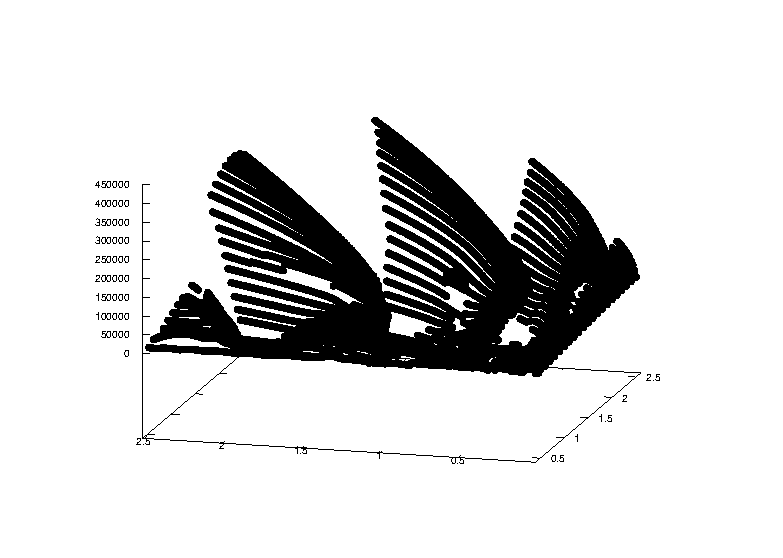
\includegraphics[width=\linewidth,angle=0]{pictures/gnuplot/3d/Hoehe/production/HoeheKraft.eps}
%	\end{center}	
%\end{figure}

\subsection{Variation des Seitenverhältnisses}

\begin{figure}[H]
	\begin{center}
		\begin{overpic}[width=\linewidth]{pictures/gnuplot/3d/svmr/production/svmr.eps}
			\put(47,3){$a/b$ [-]}
			\put(78,63){Kraft [N]}
			\put(13,34){$Mr$ [-]}
		\end{overpic}
		\caption{Maximale Kraft in Abhängigkeit des Seitenverhältnis}
		\label{fig:svmr}
	\end{center}
\end{figure}

Die Variation des Seitenverhältnisses wurde unter konstanter Fläche untersucht. Für eine gegebene Fläche $f$ und ein Seitenverhältnis $Sv$, können $a$ und $b$ wie folgt berechnet werden:

$$b = \left(\dfrac{f}{Sv}\right)^\frac{1}{2}$$
$$a = \dfrac{f}{b} $$


Es findet sich eine klare Abhängig der Stoßanzahl mit dem Seitenverhältnis. Da mit einem steigenden Seitenverhältnis unter gleicher Fläche, eine der beiden Seitenlänge minimiert wird, dominiert diese Seite die Steifigkeit der Platte. Somit erhält man ab einem Seitenverhältnis von rund 3.5 stehts nur noch einen einzigen Schlag. Ebenfalls steigt die Anzahl der Schläge mit steigenden Massenverhältnis, hat jedoch einen deutlich kleineren Einfluss als das Seitenverhältnis.
Auffallend ist zudem noch das schnelle Ansteigen der Anzahl der Schläge bei einem Seitenverhältnis zwischen 1 und 1.5. Anschließend fallen die Anzahl der Schläge wieder. Wichtig zu erwähnen ist eine numerische Instabilität des Skriptes welche bei einem Seitenverhältnis zwischen 2 und 2.5 und einem Massenverhältnis $>2$ falsche Ergebnisse erzeugt. Diese numerische Instabilität wird insbesondere ersichtlich wenn die maximale Durchbiegung aufgetragen wird.


\begin{figure}[H]
	\begin{center}
		\begin{overpic}[width=\linewidth]{pictures/gnuplot/3d/svmr/production/svmrAuslenkung.eps}
			\put(47,3){$a/b$ [-]}
			\put(87,60){Auslenkung [cm]}
			\put(13,34){$Mr$ [-]}
		\end{overpic}
		\caption{Maximale Durchbiegung in Abhängigkeit des Seitenverhältnis}
		\label{fig:svmrDurchbiegung}
	\end{center}
\end{figure}

Für eine bessere Darstellung wurde im folgenden $Mr > 2$ ignoriert. Für die Durchbiegung ergibt sich folglich:

\begin{figure}[H]
	\begin{center}
		\begin{overpic}[width=\linewidth]{pictures/gnuplot/3d/svmr/production/svmrAuslenkungFixed.eps}
			\put(47,3){$a/b$ [-]}
			\put(87,60){Auslenkung [cm]}
			\put(13,34){$Mr$ [-]}
		\end{overpic}
		\caption{Maximale Durchbiegung in Abhängigkeit des Seitenverhältnis}
		\label{fig:svmrDurchbiegungFixed}
	\end{center}
\end{figure}

Für die maximale Auslenkung sowie für die maximale Kraft ergibt sich ein ähnliches Bild. Mit steigender Impaktormasse steigt die Kraft und die Durchbiegung. Auffallend ist die eine maximale Durchbiegung für ein Seitenverhältnis von $2.5$. Dies ist insbesondere unerwartet, da die Steifigkeit der Platte für das gegebene Seitenverhältnis deutlich größer ist als für den quadratischen Fall. Es ergibt sich ebenfalls eine maximale Kraft für das soeben genannte Seitenverhältnis von $2.5$. Ab einem Seitenverhältnis $ Sv \geq 3.5$ sind die Durchbiegung und maximale Kraft homogen und weisen keine Abhängigkeit von der Masse mehr auf.   

\begin{figure}[H]
	\begin{center}
		\begin{overpic}[width=\linewidth]{pictures/gnuplot/3d/svmr/production/svmrKraftFixed.eps}
			\put(47,3){$a/b$ [-]}
			\put(87,60){Kraft [N]}
			\put(13,34){$Mr$ [-]}
		\end{overpic}
		\caption{Maximale Kraft durch in Abhängigkeit des Seitenverhältnis}
		\label{fig:svmrKraft}
	\end{center}
\end{figure}




	%Im zweiten Teil des Hauptteils folgt die Darstellung der eigenen Leistung. Aufbauend auf den im vorigen Kapitel erarbeiteten Grundlagen  wird nun der Lösungsweg aufgezeigt. Dabei wird das prinzipielle Vorgehen zum Erreichen der Zielsetzung unter Einbindung der verwendeten Hilfsmittel (Maschinen, Geräte, Programme etc. inklusive der verwendeten Einstellungen) aufgezeigt. Dabei müssen sämtliche verwendeten Daten ersichtlich sein, sodass es jederzeit möglich ist, die ermittelten Ergebnisse zu reproduzieren. Zum Schluss erfolgt unter Berücksichtigung der Randbedingungen eine kritische Analyse der Ergebnisse mit möglichen Unsicherheiten und Fehlern. Aus der Diskussion der Ergebnisse (z.B. Vergleich von Messwerten und theoretischen Vorhersagen), wird schließlich der Nutzen erörtert und mögliche weiterführende Fragestellungen werden erarbeitet.